\section{Introduction}
\subsection{Abstraction}
\begin{frame}[fragile]{\emoji{bulb} Abstraction: A Great Idea in Computer Architecture}
	Abstraction is the process of \textbf{generalizing concrete details}, away from the study of objects and systems, to \textbf{focus attention on details of greater importance}

	\onslide<2>{
		Three questions: \textbf{Why}, \textbf{What} and \textbf{How}?

		\begin{figure}
			\centering
			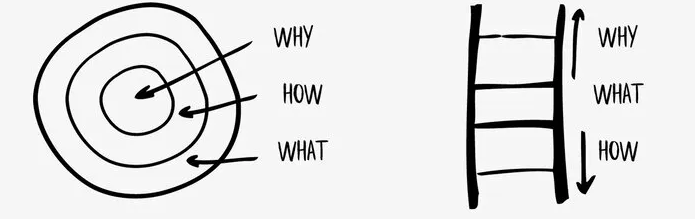
\includegraphics[width=0.8\textwidth]{day3/img/abstraction.png}
		\end{figure}
	}
\end{frame}

\subsection{Today's Topics}
\begin{frame}[fragile]{\emoji{bullseye} What we will cover today?}
	\begin{tikzpicture}[]

		% Total number of layers
		\def\numlayers{8}

		% Define layer names
		\def\layers{
			{Problem},
			{Algorithm},
			{Program},
			{Operating System},
			{ISA (Architecture)},
			{Microarchitecture},
			{Logic},
			{Circuits}
		}

		% Rectangle size
		\def\rectwidth{5}
		\def\rectheight{0.8}

		\only<1>{
			% Draw each layer with overlay
			\foreach \layer [count=\i from 0] in \layers {
				\pgfmathsetmacro{\y}{-\i * \rectheight}
				\def\fillcolor{white}
				\draw[line width=1pt, fill=\fillcolor]
				(-\rectwidth/2, \y) rectangle (\rectwidth/2, \y - \rectheight);
				\node[font=\bfseries\sffamily] at (0, \y - 0.5*\rectheight) {\layer};
			}
		}

		\only<2>{
			% Draw each layer with overlay
			\foreach \layer [count=\i from 0] in \layers {
				\pgfmathsetmacro{\y}{-\i * \rectheight}
				% Determine fill color
				\ifnum\i=0
					\def\fillcolor{blue!20}
					\def\textcolor{blue!70!black}
				\else\ifnum\i=1
						\def\fillcolor{blue!20}
						\def\textcolor{blue!70!black}
					\else
						\def\fillcolor{white}
						\def\textcolor{black}
					\fi\fi
				\draw[line width=1pt, fill=\fillcolor]
				(-\rectwidth/2, \y) rectangle (\rectwidth/2, \y - \rectheight);
				\node[font=\bfseries\sffamily, color=\textcolor] at (0, \y - 0.5*\rectheight) {\layer};
			}

			% Coordinates for Problem and Algorithm layers
			\coordinate (start) at ($(3, -0.5*\rectheight)$);
			\coordinate (end) at ($(3, -1.5*\rectheight)$);
			% Draw arrow
			\draw[->, ultra thick, black!70!black] (start) -- (end);
			% Annotation on the right
			\node[anchor=west, align=left] at ($(start)!0.5!(end) + (0.2,0)$) {Programming Languages: C, C++ (OOP), Java\\Algorithms: FDS, ADS, Operations Research};

			\node[inner sep=0pt] (picture) at ($(start)!0.5!(end) + (4.6,-3)$)
			{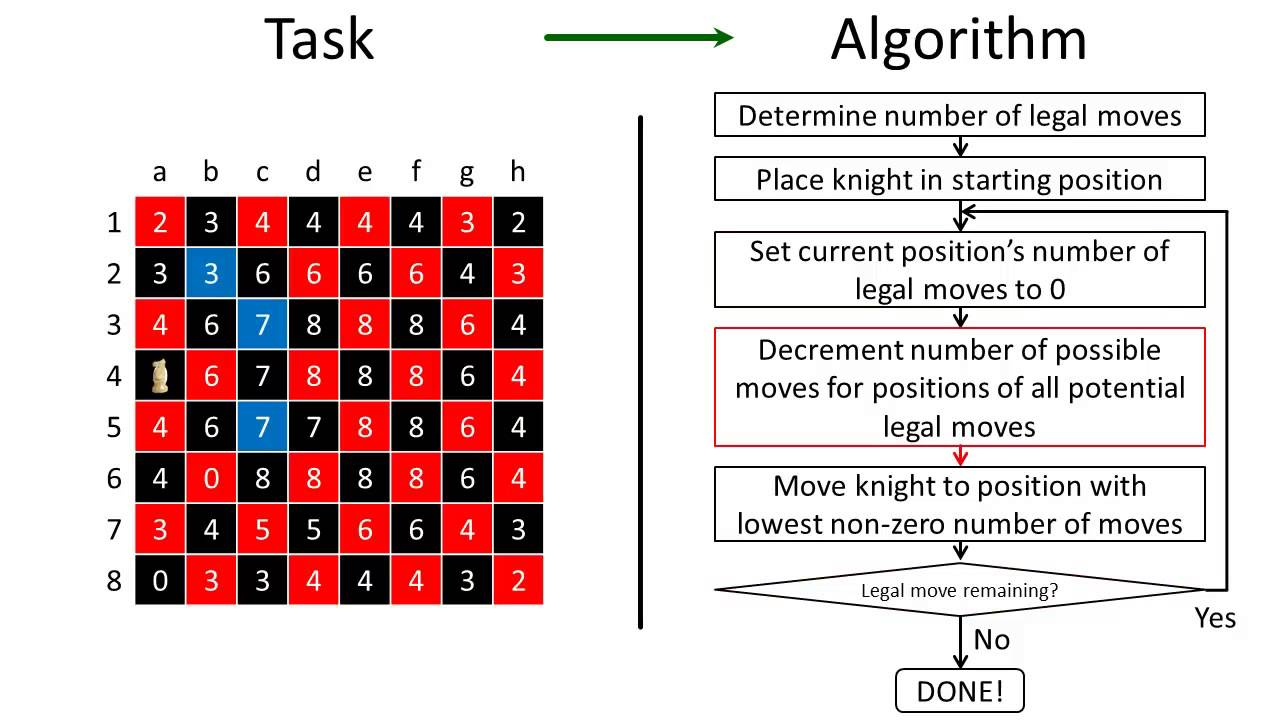
\includegraphics[width=.6\textwidth]{day3/img/prob-algo.jpg}};
		}

		\only<3>{
			\def\layers{
				{Problem},
				{Algorithm (Code)},
				{Program (Executable)},
				{Runtime System},
				{ISA (Architecture)},
				{Microarchitecture},
				{Logic},
				{Circuits}
			}
			% Draw each layer with overlay
			\foreach \layer [count=\i from 0] in \layers {
				\pgfmathsetmacro{\y}{-\i * \rectheight}
				% Determine fill color
				\ifnum\i=1
					\def\fillcolor{blue!20}
					\def\textcolor{blue!70!black}
				\else\ifnum\i=2
						\def\fillcolor{blue!20}
						\def\textcolor{blue!70!black}
					\else
						\def\fillcolor{white}
						\def\textcolor{black}
					\fi\fi
				\draw[line width=1pt, fill=\fillcolor]
				(-\rectwidth/2, \y) rectangle (\rectwidth/2, \y - \rectheight);
				\node[font=\bfseries\sffamily, color=\textcolor] at (0, \y - 0.5*\rectheight) {\layer};
			}

			% Coordinates for Problem and Algorithm layers
			\coordinate (start) at ($(3, -1.5*\rectheight)$);
			\coordinate (end) at ($(3, -2.5*\rectheight)$);
			% Draw arrow
			\draw[->, ultra thick, black!70!black] (start) -- (end);
			% Annotation on the right
			\node[anchor=west, align=left] at ($(start)!0.5!(end) + (0.2,0)$) {Compiler Principles\\GCC, LLVM (clang, Intel OneAPI, Bisheng)};

			\node[inner sep=0pt] (picture) at ($(start)!0.5!(end) + (2,-3)$)
			{
\includegraphics[width=.2\textwidth]{day3/img/llvm.png}};
			\node[inner sep=0pt] (picture) at ($(start)!0.5!(end) + (4.6,-3)$)
			{
\includegraphics[width=.2\textwidth]{day3/img/oneapi.png}};
			\node[inner sep=0pt] (picture) at ($(start)!0.5!(end) + (7.6,-3)$)
			{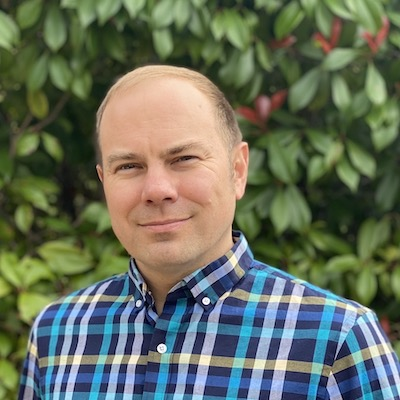
\includegraphics[width=.2\textwidth]{day3/img/chris.jpg}};
		}

		\only<4>{
			% Draw each layer with overlay
			\foreach \layer [count=\i from 0] in \layers {
				\pgfmathsetmacro{\y}{-\i * \rectheight}
				% Determine fill color
				\ifnum\i=2
					\def\fillcolor{blue!20}
					\def\textcolor{blue!70!black}
				\else\ifnum\i=3
						\def\fillcolor{blue!20}
						\def\textcolor{blue!70!black}
					\else
						\def\fillcolor{white}
						\def\textcolor{black}
					\fi\fi
				\draw[line width=1pt, fill=\fillcolor]
				(-\rectwidth/2, \y) rectangle (\rectwidth/2, \y - \rectheight);
				\node[font=\bfseries\sffamily, color=\textcolor] at (0, \y - 0.5*\rectheight) {\layer};

				\node[inner sep=0pt] (picture) at ($(start)!0.5!(end) + (4,-3.1)$)
				{
\includegraphics[width=.28\textwidth]{day3/img/os-meme.png}};
			}

			% Coordinates for Problem and Algorithm layers
			\coordinate (start) at ($(3, -2.5*\rectheight)$);
			\coordinate (end) at ($(3, -3.5*\rectheight)$);
			% Draw arrow
			\draw[->, ultra thick, black!70!black] (start) -- (end);
			% Annotation on the right
			\node[anchor=west, align=left] at ($(start)!0.5!(end) + (0.2,0)$) {Operating System / Computer System III};
		}

		\only<5>{
			% Draw each layer with overlay
			\foreach \layer [count=\i from 0] in \layers {
				\pgfmathsetmacro{\y}{-\i * \rectheight}
				% Default colors
				\def\fillcolor{white}
				\def\textcolor{black}

				% Override for specific layers
				\ifnum\i=3
					\def\fillcolor{blue!20}
					\def\textcolor{blue!70!black}
				\fi
				\ifnum\i=4
					\def\fillcolor{blue!20}
					\def\textcolor{blue!70!black}
				\fi
				\ifnum\i=5
					\def\fillcolor{blue!20}
					\def\textcolor{blue!70!black}
				\fi
				\draw[line width=1pt, fill=\fillcolor]
				(-\rectwidth/2, \y) rectangle (\rectwidth/2, \y - \rectheight);
				\node[font=\bfseries\sffamily, color=\textcolor] at (0, \y - 0.5*\rectheight) {\layer};

				\node[inner sep=0pt] (picture) at ($(start)!0.5!(end) + (4.2,1)$)
				{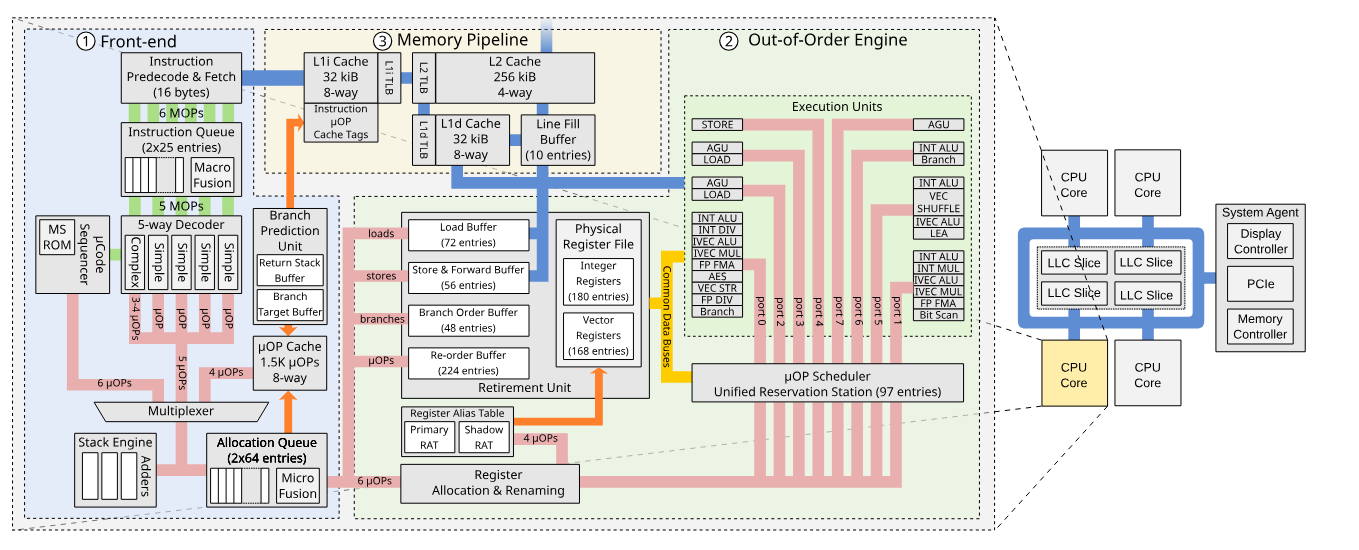
\includegraphics[width=.55\textwidth]{day3/img/uarch.png}};
			}

			% Coordinates for Problem and Algorithm layers
			\coordinate (start) at ($(3, -3.5*\rectheight)$);
			\coordinate (end) at ($(3, -5.5*\rectheight)$);
			% Draw arrow
			\draw[->, ultra thick, black!70!black] (start) -- (end);
			% Annotation on the right
			\node[anchor=west, align=left] at ($(start)!0.5!(end) + (0.2,0)$) {Computer Architecture \& Computer Organization\\Computer System II};
		}

		\only<6>{
			% Draw each layer with overlay
			\foreach \layer [count=\i from 0] in \layers {
				\pgfmathsetmacro{\y}{-\i * \rectheight}
				% Default colors
				\def\fillcolor{white}
				\def\textcolor{black}

				% Override for specific layers
				\ifnum\i=5
					\def\fillcolor{blue!20}
					\def\textcolor{blue!70!black}
				\fi
				\ifnum\i=6
					\def\fillcolor{blue!20}
					\def\textcolor{blue!70!black}
				\fi
				\ifnum\i=7
					\def\fillcolor{blue!20}
					\def\textcolor{blue!70!black}
				\fi
				\draw[line width=1pt, fill=\fillcolor]
				(-\rectwidth/2, \y) rectangle (\rectwidth/2, \y - \rectheight);
				\node[font=\bfseries\sffamily, color=\textcolor] at (0, \y - 0.5*\rectheight) {\layer};
			}

			% Coordinates for Problem and Algorithm layers
			\coordinate (start) at ($(3, -5.5*\rectheight)$);
			\coordinate (end) at ($(3, -7.5*\rectheight)$);
			% Draw arrow
			\draw[->, ultra thick, black!70!black] (start) -- (end);
			% Annotation on the right
			\node[anchor=west, align=left] at ($(start)!0.5!(end) + (0.2,0)$) {Digital Logic Design / Computer System I};
			\node[inner sep=0pt] (picture) at ($(start)!0.5!(end) + (4.3,3)$)
			{
\includegraphics[width=.55\textwidth]{day3/img/turing.jpg}};
		}

		\only<7>{
			% Draw each layer with overlay
			\foreach \layer [count=\i from 0] in \layers {
				\pgfmathsetmacro{\y}{-\i * \rectheight}
				% Default colors
				\def\fillcolor{white}
				\def\textcolor{black}

				% Override for specific layers
				\ifnum\i=2
					\def\fillcolor{blue!20}
					\def\textcolor{blue!70!black}
				\fi
				\ifnum\i=3
					\def\fillcolor{blue!20}
					\def\textcolor{blue!70!black}
				\fi
				\ifnum\i=4
					\def\fillcolor{blue!20}
					\def\textcolor{blue!70!black}
				\fi
				\ifnum\i=5
					\def\fillcolor{blue!20}
					\def\textcolor{blue!70!black}
				\fi
				\draw[line width=1pt, fill=\fillcolor]
				(-\rectwidth/2, \y) rectangle (\rectwidth/2, \y - \rectheight);
				\node[font=\bfseries\sffamily, color=\textcolor] at (0, \y - 0.5*\rectheight) {\layer};
			}

			% Coordinates for Problem and Algorithm layers
			\coordinate (start) at ($(3, -2.5*\rectheight)$);
			\coordinate (end) at ($(3, -5.5*\rectheight)$);
			% Draw arrow
			\draw[->, ultra thick, black!70!black] (start) -- (end);
			% Annotation on the right
			\node[anchor=west, align=left] at ($(start)!0.5!(end) + (0.2,0)$) {Our Focus in\\\emph{Introduction to Computer Systems in HPC}\\Day 1: \textbf{Operating System (TLP)}\\Day 2: \textbf{Computer Architecture (DLP)}};
		}

	\end{tikzpicture}
\end{frame}
